\clearpage
%%=========================================
\section[Surface Analysis of Substrate B with Surface Pre-Growth Preparation]{Surface Analysis of Substrate B with Surface Pre-Growth Preparation%
   \sectionmark{Surface Analysis of Pre-Growth Substrate B}}\sectionmark{Surface Analysis of Pre-Growth Substrate B}\label{sec:subBb}
   
The dark field images taken of the surface of substrate B after polishing and etching show that the surface pre-growth preparation has improved the surface considerably, see Fig.~\ref{fig:subBa_om_df} and Fig.~\ref{fig:subBb_om_df}. The previously observed deep surface scratches are removed and there are far less particles and other features on the substrate surface. In comparison to substrate B, substrate B2 have more particles larger than \SI{0.5}{\micro\metre} on the surface, but it too are without deep surface scratches and large features, see Fig.~\ref{fig:subB2b_om_df}.

\begin{figure}[htbp]
    \centering
    \begin{subfigure}[t]{0.8\linewidth}
    
\includegraphics[width=\linewidth]{subBb_om_n016.jpg}
    \caption{Substrate B -- near the upper left corner.}\label{fig:subBb_om_df}
    \end{subfigure}
    \par\bigskip
    \begin{subfigure}[t]{0.8\linewidth}
    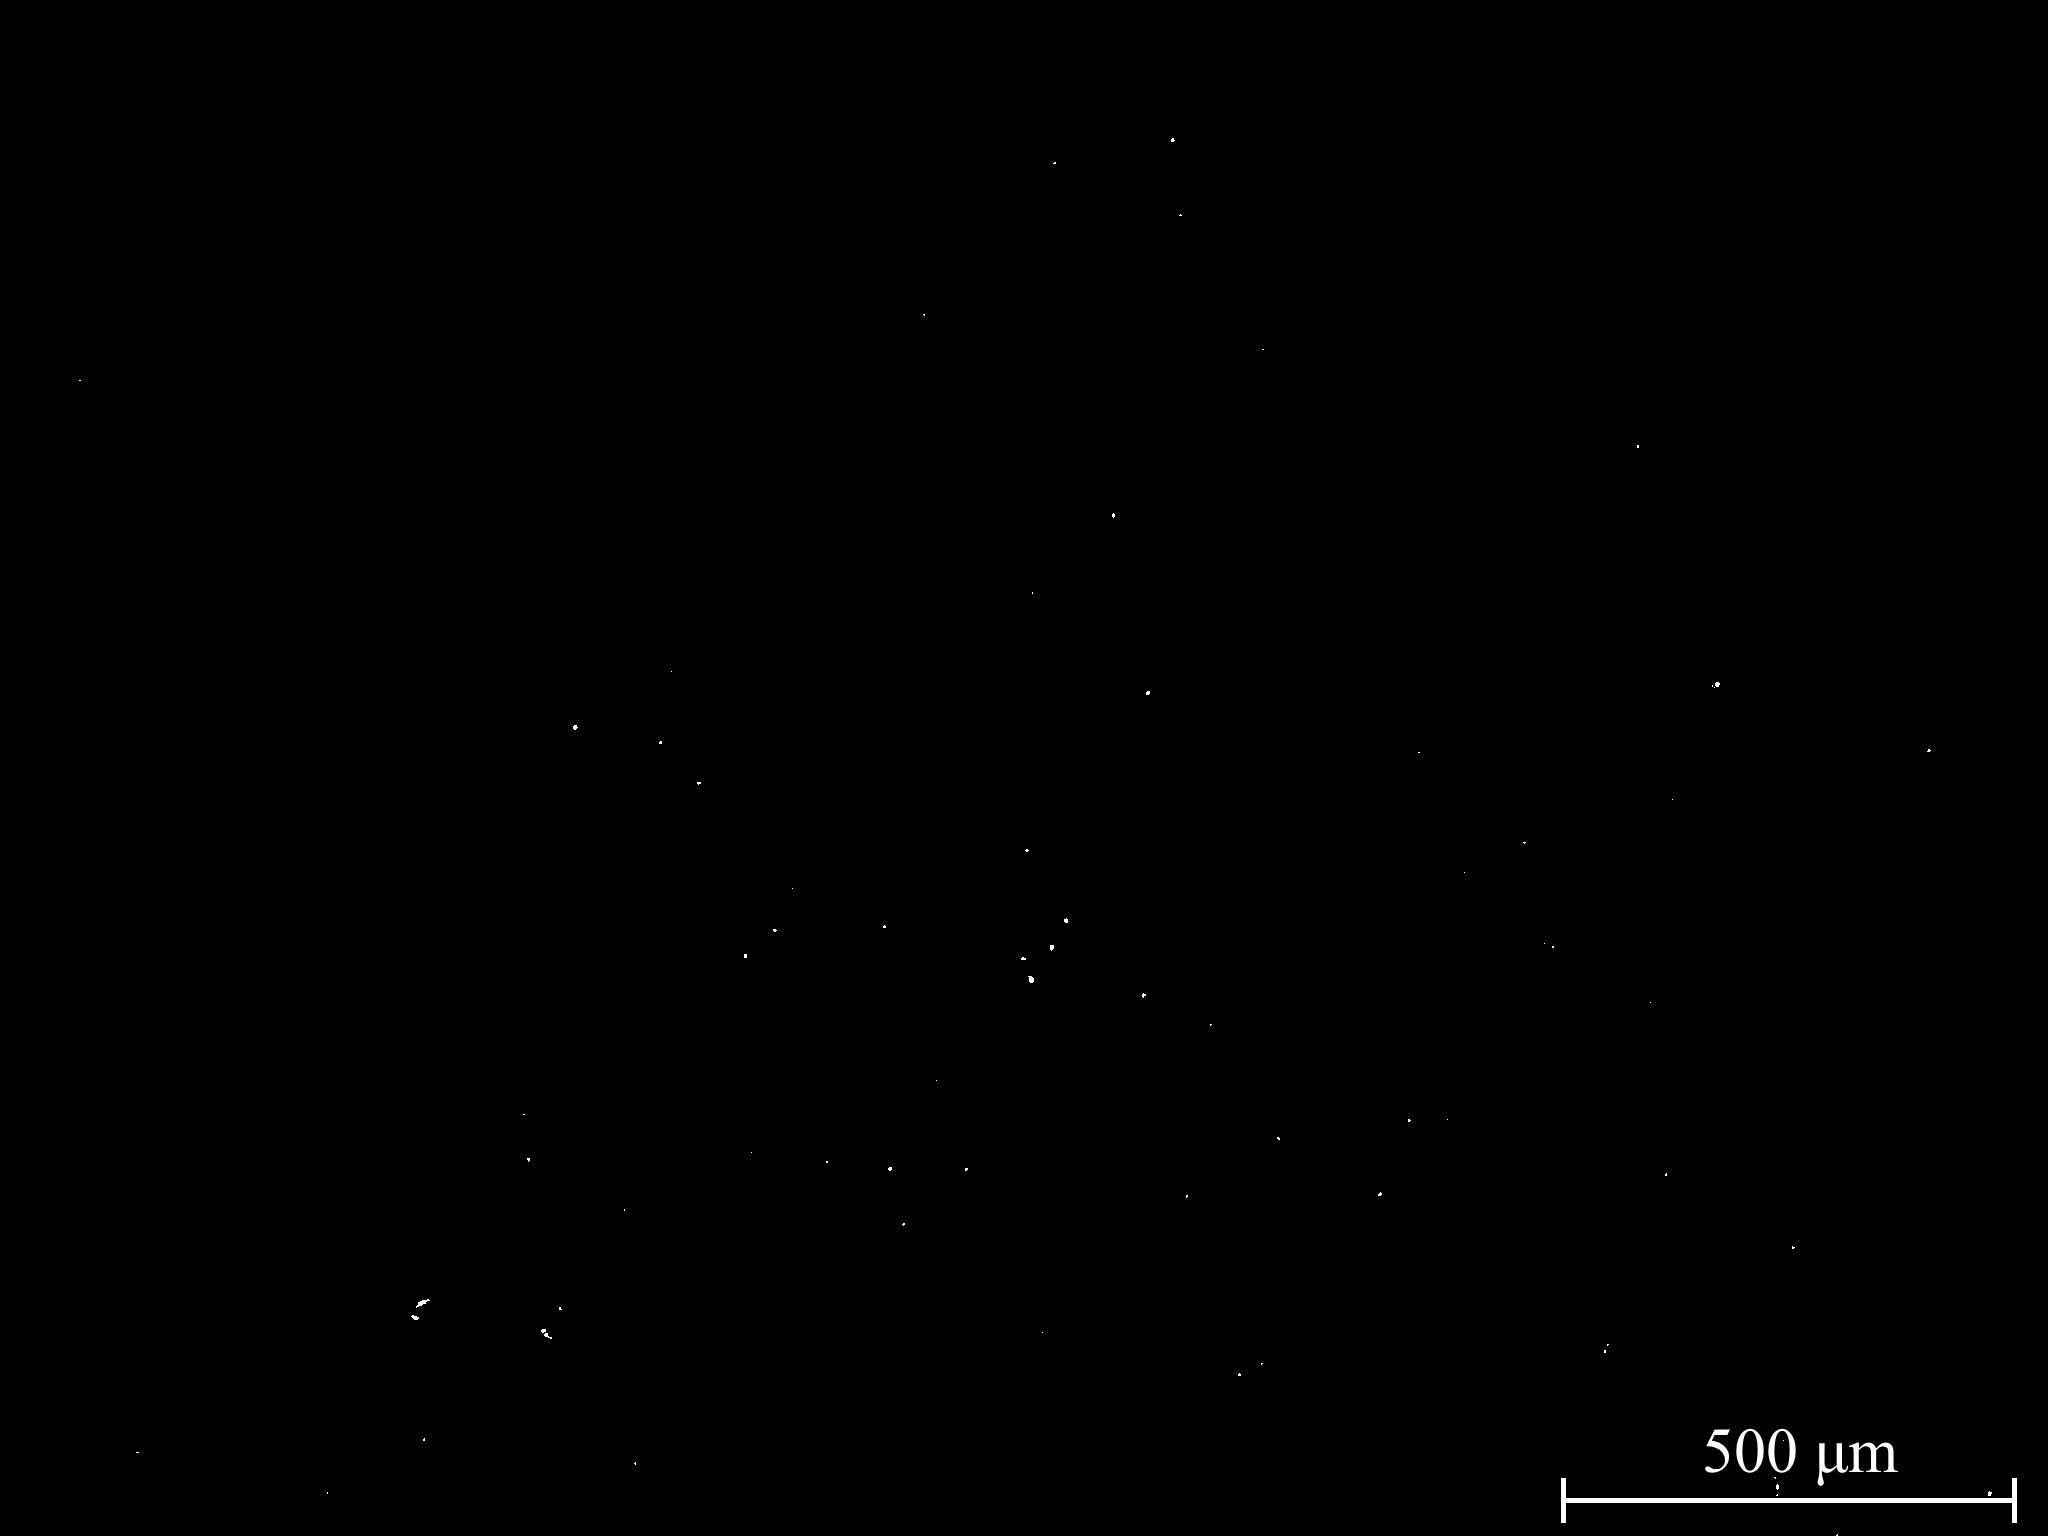
\includegraphics[width=\linewidth]{subB2b_om_5x_n022.jpg}
    \caption{Substrate B2 -- near the centre.}\label{fig:subB2b_om_df}
    \end{subfigure}
    \caption[Dark field optical microscopy image of substrate B and B2 with surface pre-growth preparation.]{Dark field optical microscopy image of substrate B and B2 with surface pre-growth preparation taken in the upper left corner and near the centre of the substrate respectively at a magnification of $5\times$.}\label{fig:subBb_and_subB2b_om_df}
\end{figure}

\Ac{sem} shows the surface at a higher magnification and reveals that there are much smaller particles distributed over the surface as well. A typical area in the centre of substrate B and substrate B2 can be seen in Fig.~\ref{fig:subBb_sem_typical_centre} and Fig.~\ref{fig:subB2b_sem_typical_centre} respectively. The particle density in the two images are \SI{2e+08}{\particle\centi\metre^{-2}} and \SI{6e+07}{\particle\centi\metre^{-2}} respectively. The particles have lengths of \SIrange{20}{50}{\nano\metre}. 

%Here the particle density is  \SI{\sim 2e+06}{\particle\centi\metre^{-2}}. The highest observed density of particles is counted near the upper edge to be \SI{3e+07}{\particle\centi\metre^{-2}}, see Fig.~\ref{fig:subAb_sem_typical_edge}. 

\begin{figure}[htbp]
    \begin{subfigure}[t]{0.49\textwidth}
        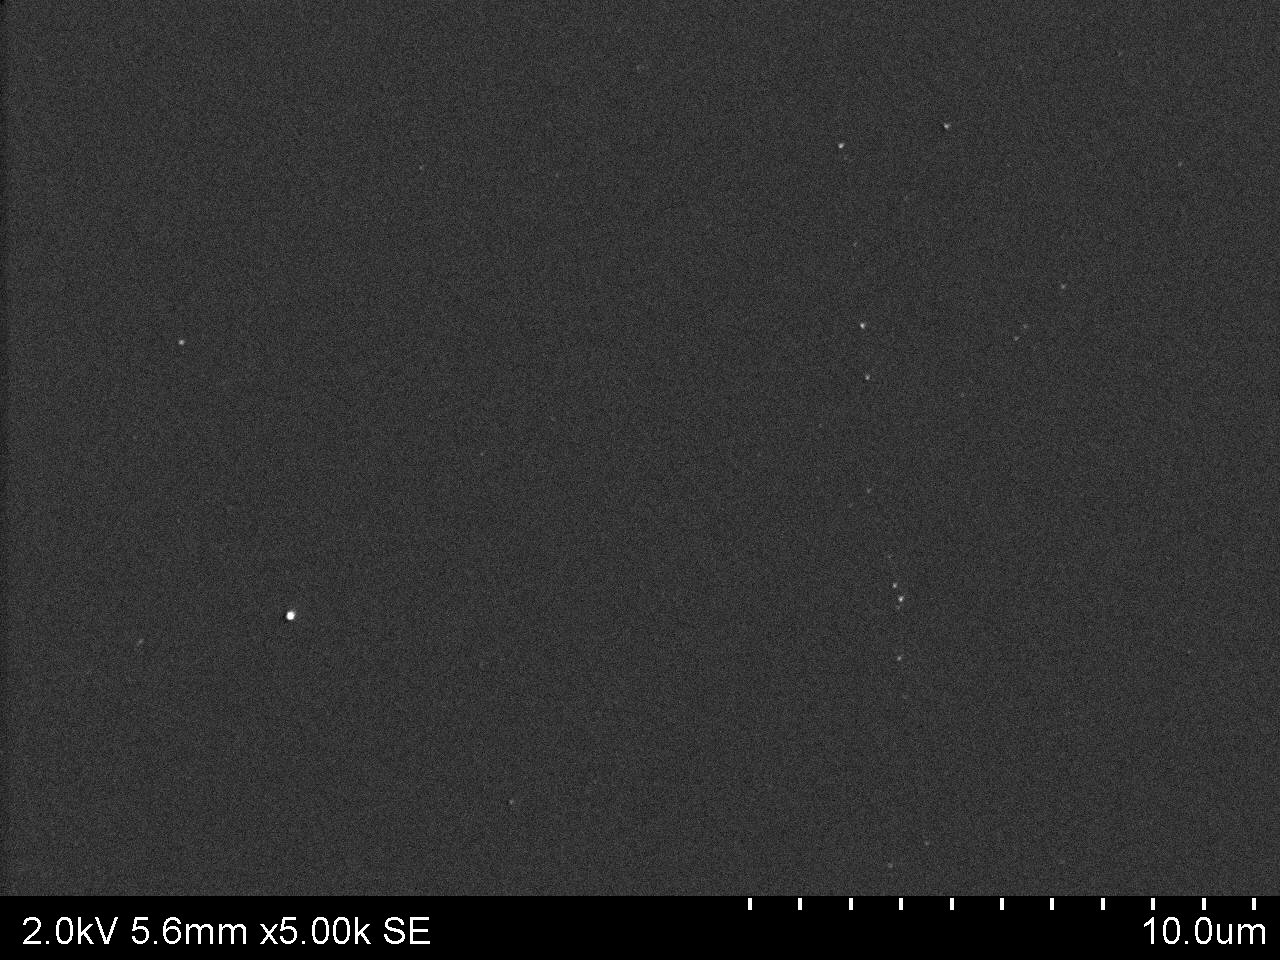
\includegraphics[width=\linewidth]{subBb_sem_05a_m014.jpg}
        \caption{Substrate B}\label{fig:subBb_sem_typical_centre}
    \end{subfigure}%
    \hfill
    \begin{subfigure}[t]{0.49\textwidth}
        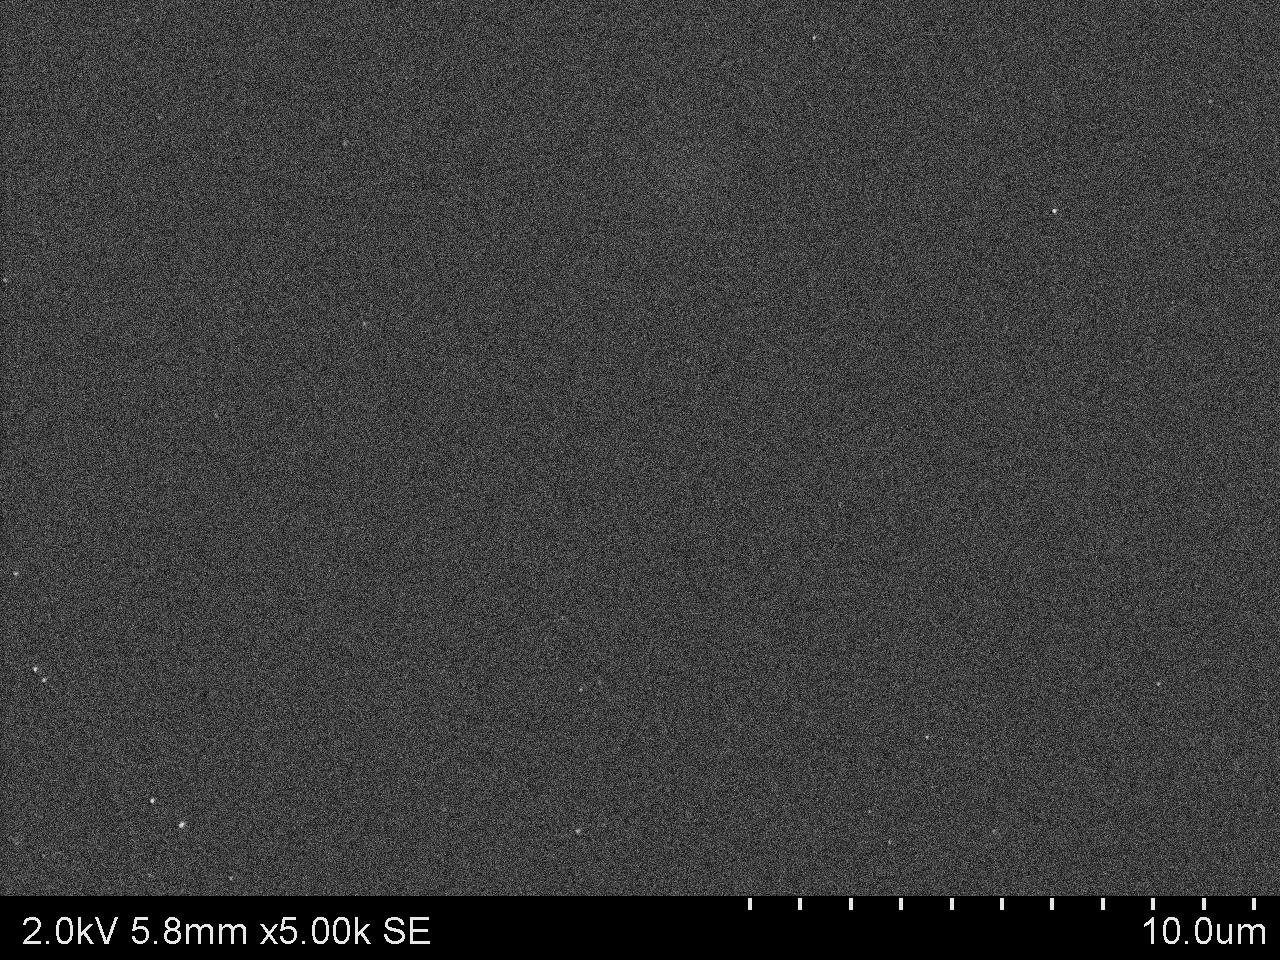
\includegraphics[width=\linewidth]{subB2b_sem_02b_m004.jpg}
        \caption{Substrate B2}\label{fig:subB2b_sem_typical_centre}
    \end{subfigure}%
    \caption[\Ac{sem} images of typical areas on substrate B and B2 with surface pre-growth preparation.]{\Acf{sem} images of a typical area near the centre of substrate B and substrate B2 after surface pre-growth preparation taken at a magnification of $5000\times$.}\label{fig:subBb_and_subB2b_sem_typical}
\end{figure}

%%=========================================
% Twin boundaries.
Four twin boundaries are visible to the naked eye after polish and etch. Two in the upper left corner and two that span from the lower right corner to the middle of the upper edge, see Fig.~\ref{fig:subBb_twins_illustration}. By doing an \todo{spør Espen om navn på etch} etch it was established that the area between the lines in the upper left corner and between the two other lines were (111)B-oriented, while the surrounding area were twins. A part of the twin boundary near the upper left corner can be seen in Fig.~\ref{fig:subBb_sem_twins}. It forms a piecewise straight line with steps that change the direction by \SI{\pm 45}{\degree} every \SIrange{10}{200}{\micro\metre}.

\citet{ashida2015crystallographic} studied the dependence of \ac{sem} contrast on crystallographic orientation in \ce{SiC} polytypes. They found that features look brighter when the direction of the incident electron beam is almost parallel to the topmost stacking sequence direction. However, the formation mechanism of the \ac{sem} contrast is still under discussion. This explains why there is a visible contrast at the twin boundaries.

\begin{figure}[htbp]
    \centering
    \begin{subfigure}[t]{0.4\linewidth}
        \centering
        \begin{tikzpicture}[remember picture]
          \node[anchor=south west,inner sep=0] (imageA) {
\includegraphics[width=\linewidth]{subBb_twins.png}};
          \begin{scope}[x={(imageA.south west)},y={(imageA.north east)}]
            \node[coordinate] (A) at (0.1\linewidth, 0.9\linewidth) {};
          \end{scope}
        \end{tikzpicture}
    \caption{Location of twin boundaries.}\label{fig:subBb_twins_illustration}
    \end{subfigure}
    \hfill
    \begin{subfigure}[t]{0.5333\linewidth}
    \centering
        \begin{tikzpicture}[remember picture]
          \node[anchor=south west,inner sep=0] (imageB) {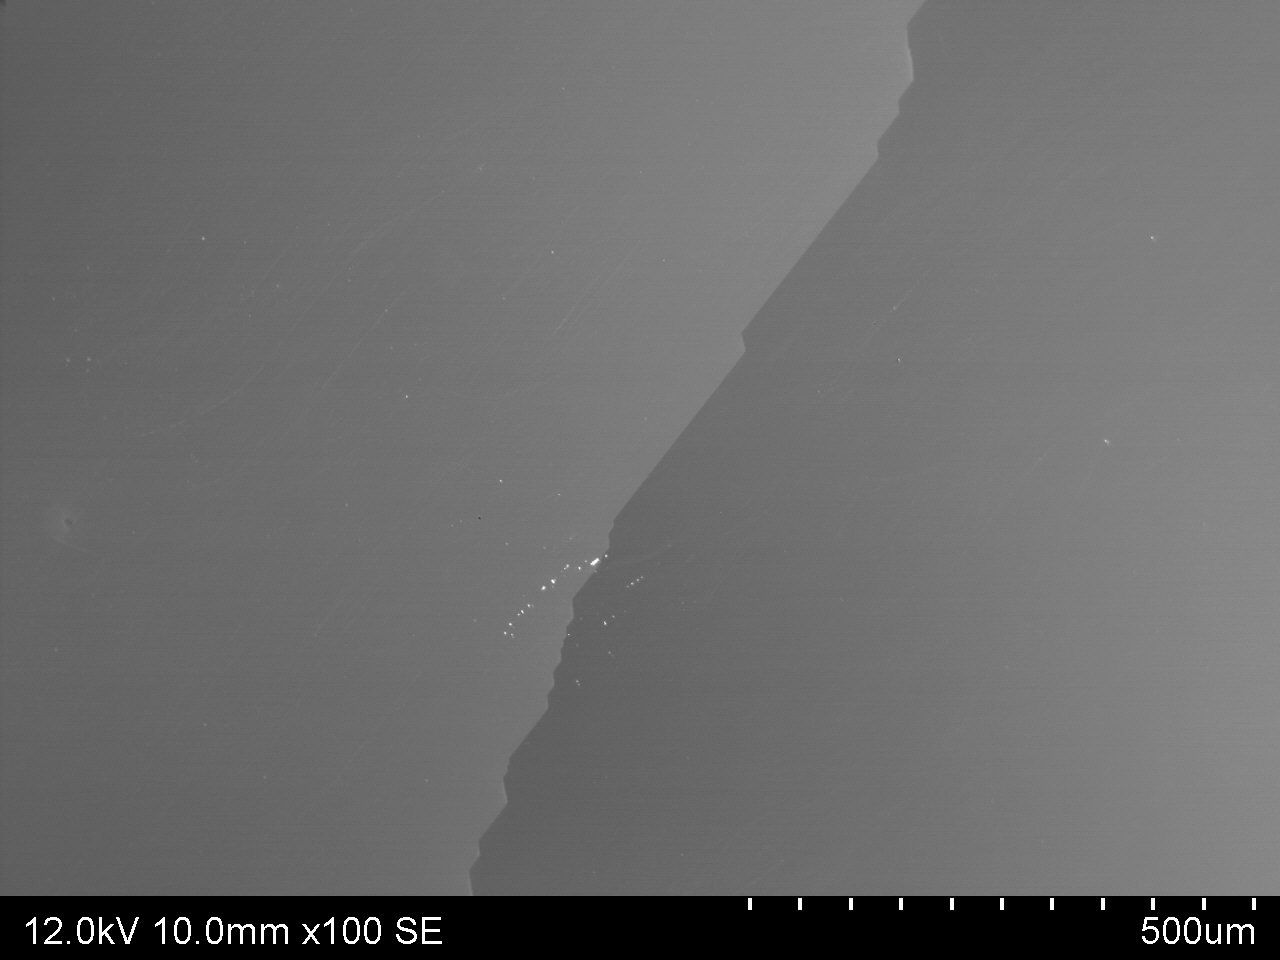
\includegraphics[width=\linewidth]{subBb_sem_01_m005.jpg}};
          \begin{scope}[x={(imageB.south west)},y={(imageB.north east)}]
            \node[coordinate] (B) at (0.5,0.5) {};
          \end{scope}
        \end{tikzpicture}
    \caption{\Ac{sem} image of twin boundary near the upper left corner.}\label{fig:subBb_sem_twins}
    \end{subfigure}
    \caption[Twin boundaries on substrate B.]{Twin boundaries on substrate B.}\label{fig:subBb_twin_boundaries}
\end{figure}
% Draw arrow.
\begin{tikzpicture}[remember picture,overlay]
  \draw[->, red, line width=0.5mm ] (B) -- (A);
\end{tikzpicture}

%%=========================================
\subsection{Particles}

Four different types of particles were observed on the surface of substrate B and substrate B2 after surface pre-growth preparation, see Fig.~\ref{fig:subBb_sem_w_eds}. They will be described and identified in the following.

\begin{figure}[htbp]
    \centering
    \begin{subfigure}[t]{\textwidth}
          \begin{minipage}[t]{0.49\linewidth}
            \centering
            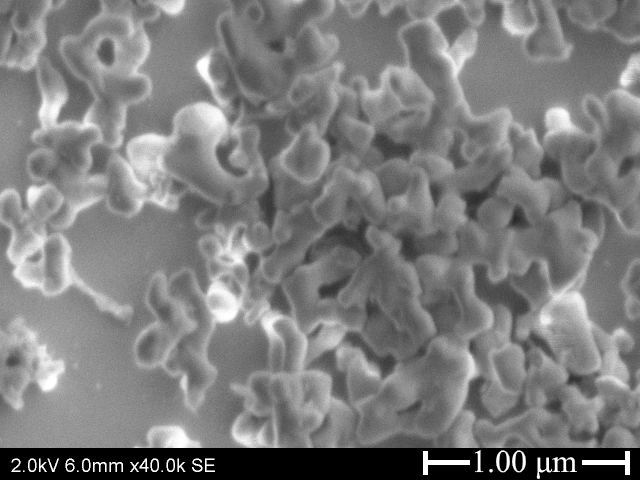
\includegraphics[width=\linewidth]{subB2b_sem_03_m006.png}
          \end{minipage}
          \hfill
          \begin{minipage}[t]{0.49\linewidth}
            \centering
            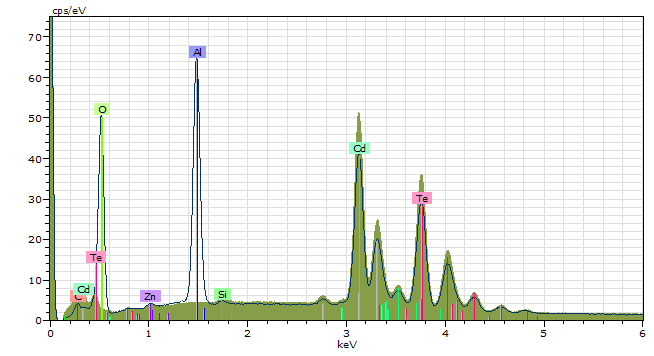
\includegraphics[width=\linewidth]{subB2b_sem_03_m006_eds.png}
          \end{minipage}
        \caption{Alumina (\ce{Al2O3}) polishing grit agglomeration.}\label{fig:subB2b_alumina}
    \end{subfigure}
    \par\bigskip
    \begin{subfigure}[t]{\textwidth}
          \begin{minipage}[t]{0.49\linewidth}
            \centering
            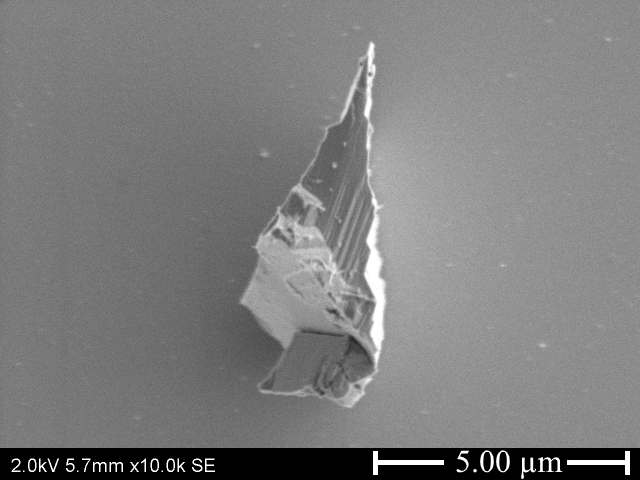
\includegraphics[width=\linewidth]{subB2b_sem_03_m002.png}
          \end{minipage}
          \hfill
          \begin{minipage}[t]{0.49\linewidth}
            \centering
            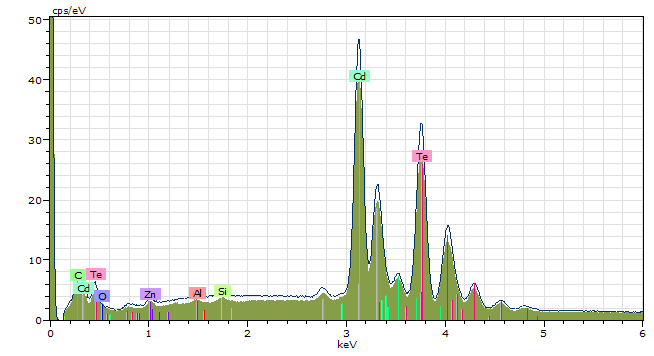
\includegraphics[width=\linewidth]{subB2b_sem_03_m002_eds.png}
          \end{minipage}
        \caption{\Ac{czt} particle.}\label{fig:subB2b_czt}
    \end{subfigure}
    \par\bigskip
    \begin{subfigure}[t]{\textwidth}
          \begin{minipage}[t]{0.49\linewidth}
            \centering
            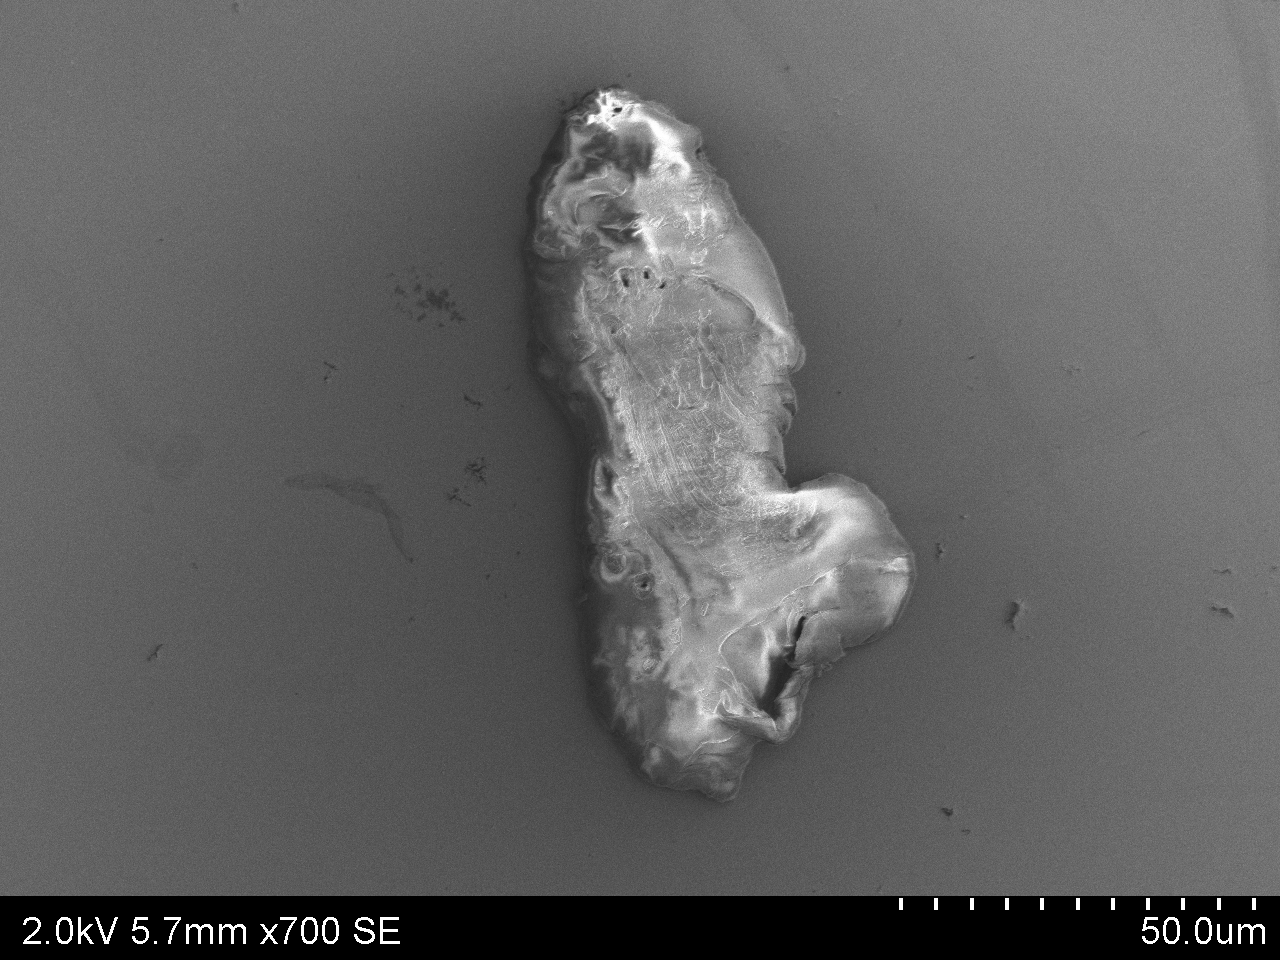
\includegraphics[width=\linewidth]{subB2b_sem_03_m001.png}
          \end{minipage}
          \hfill
          \begin{minipage}[t]{0.49\linewidth}
            \centering
            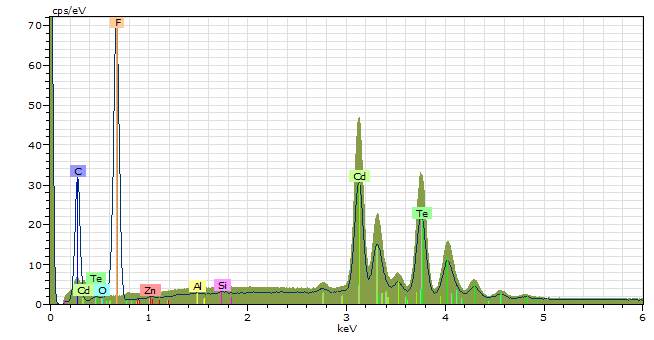
\includegraphics[width=\linewidth]{subB2b_sem_03_m001_eds.png}
          \end{minipage}
        \caption{Particle based on \SI{\sim 5}{} flouride (\ce{F}) and \SI{\sim 2}{} carbon (\ce{C}).}\label{fig:subB2b_C2F5}
    \end{subfigure}
    \caption[\Ac{sem} images and \ac{eds} spectra of particles found on substrate B and substrate B2 after surface pre-growth preparation.]{High resolution \acf{sem} images of particles found on substrate B and substrate B2 after surface pre-growth preparation and the corresponding \acf{eds} spectra of the particles.}\label{fig:subBb_sem_w_eds}
\end{figure}

\begin{figure}[htbp]
\ContinuedFloat
    \centering
    \begin{subfigure}[t]{\textwidth}
          \begin{minipage}[t]{0.49\linewidth}
            \centering
            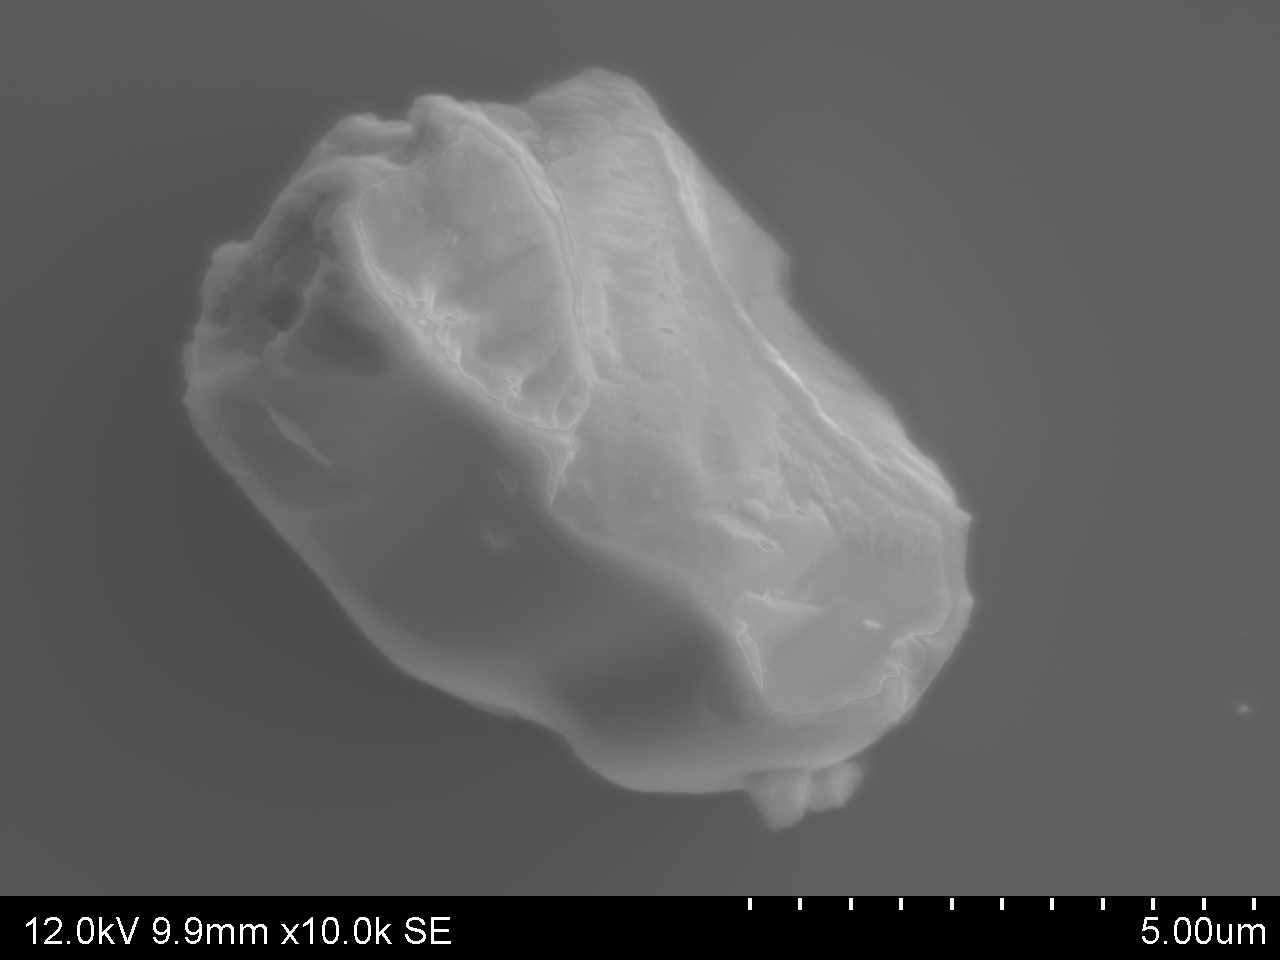
\includegraphics[width=\linewidth]{subB2b_sem_04_m010.png}
          \end{minipage}
          \hfill
          \begin{minipage}[t]{0.49\linewidth}
            \centering
            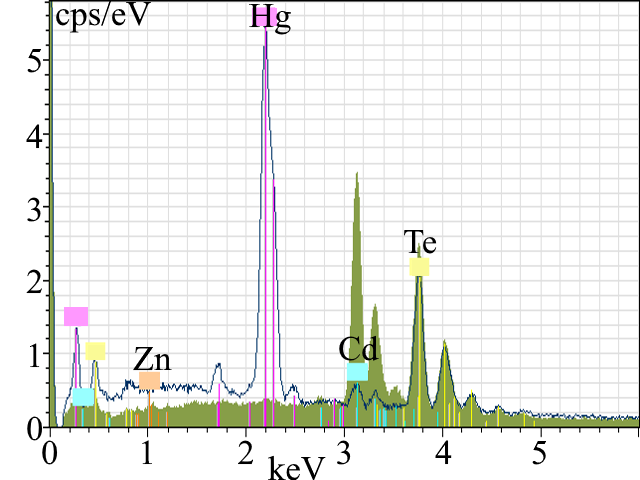
\includegraphics[width=\linewidth]{subB2b_sem_04_m010_eds.png}
          \end{minipage}
        \caption{\Ac{mct} particle}\label{fig:subB2b_mct}
    \end{subfigure}
    \captionsetup{list=no}
    \caption{\emph{(continued)}}
\end{figure}

The small particles observed in \ac{sem} are distributed evenly over the surface with a tendency of higher density towards the upper right, lower right, and lower left corners. The particle density was found to be between \SI{5e+06}{\particle\centi\metre^{-2}} and \SI{5e+07}{\particle\centi\metre^{-2}}. The mean particle density was \SI{2e+07}{\particle\centi\metre^{-2}} with a standard deviation of \SI{9e+06}{\particle\centi\metre^{-2}}. A graphical representation of the particle density at different locations on substrate B can be seen in Fig.~\ref{fig:subBb_densityData}.

Substrate B2 have a similar distribution of polishing grit. There are higher densities of particles near the left and upper edges. The particle density was found to be between \SI{3e+06}{\particle\centi\metre^{-2}} and \SI{7e+07}{\particle\centi\metre^{-2}}. The mean particle density was \SI{2e+07}{\particle\centi\metre^{-2}}, the same as for substrate B, with a standard deviation of \SI{2e+07}{\particle\centi\metre^{-2}}. A graphical representation of the particle density at different locations on substrate B2 can be seen in Fig.~\ref{fig:subB2b_densityData}.

\begin{figure}[htbp]
    \centering
    \begin{subfigure}[t]{0.8\textwidth}
        \centering
        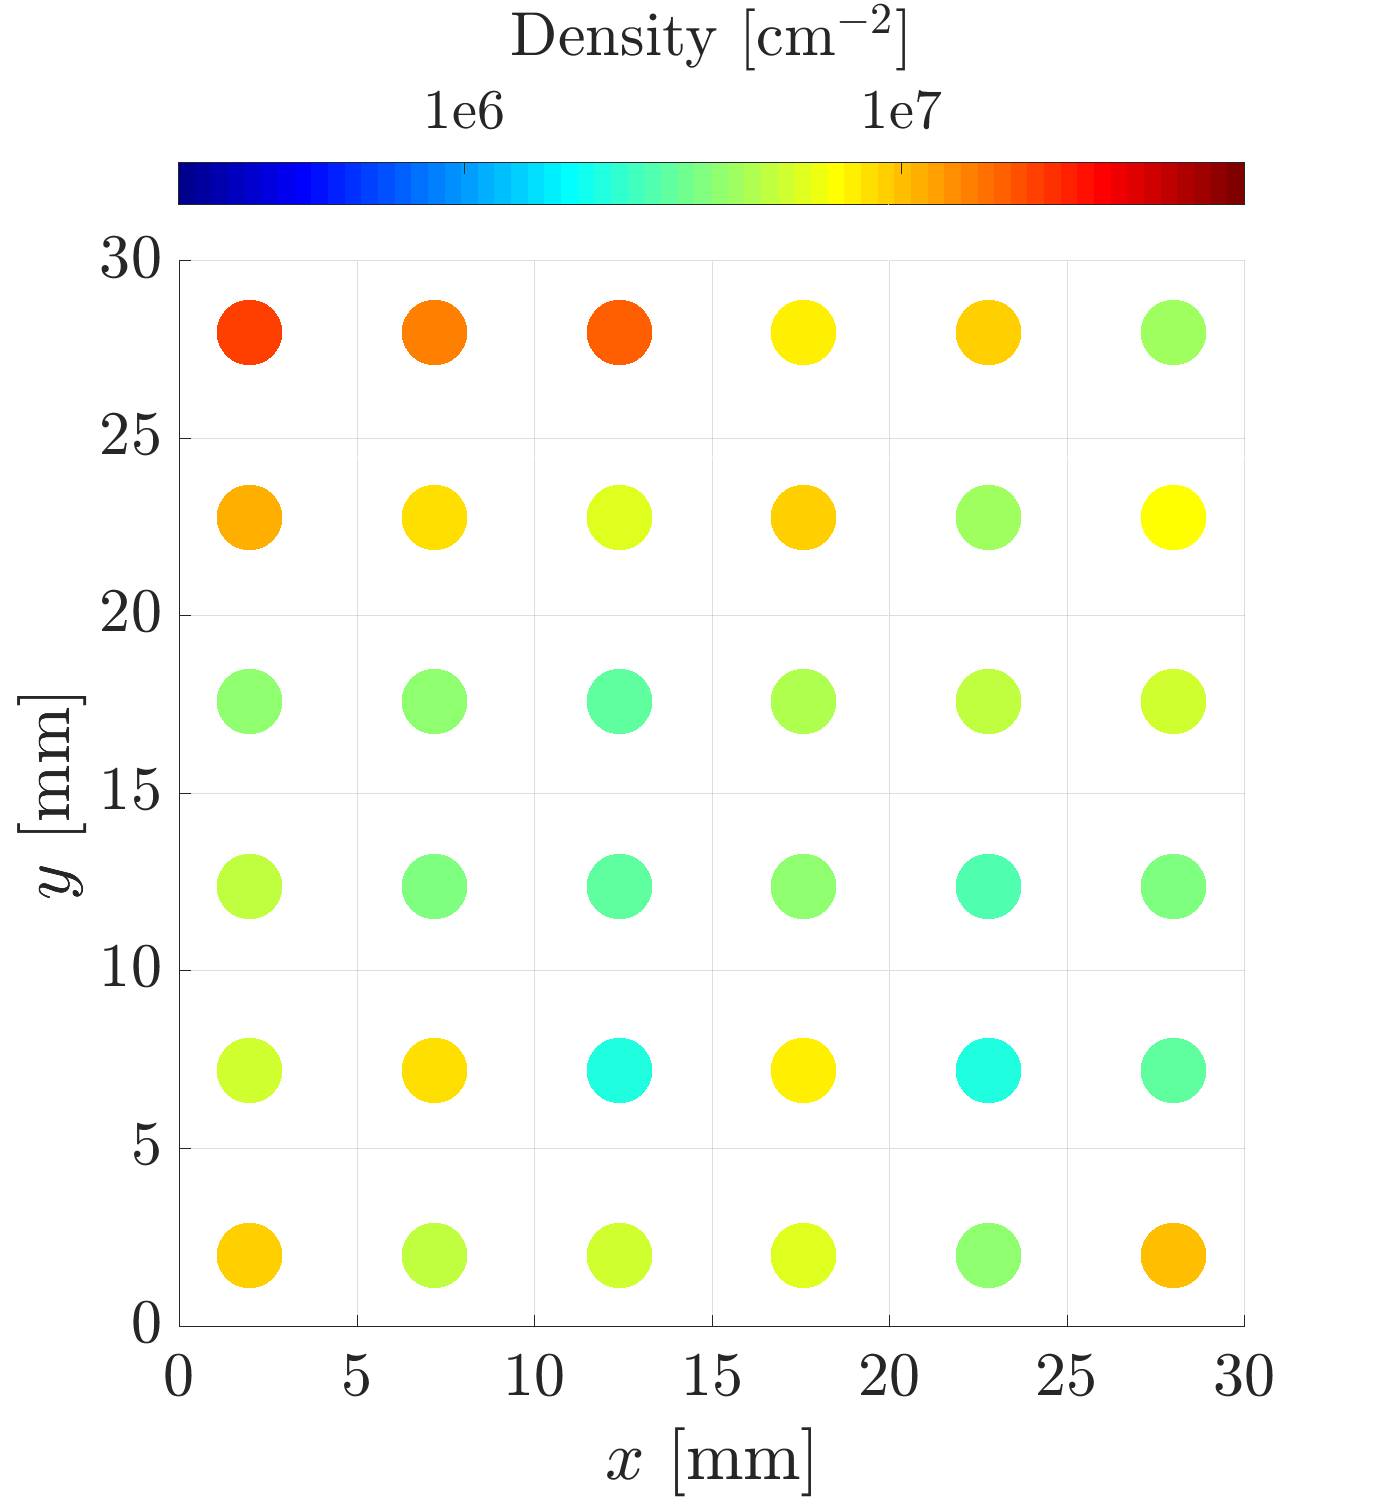
\includegraphics[width=\linewidth]{subBb_densityData.png}
        \caption{Substrate B with surface pre-growth preparation.}\label{fig:subBb_densityData}
    \end{subfigure}
    \par\bigskip
    \begin{subfigure}[t]{0.8\textwidth}
        \centering
        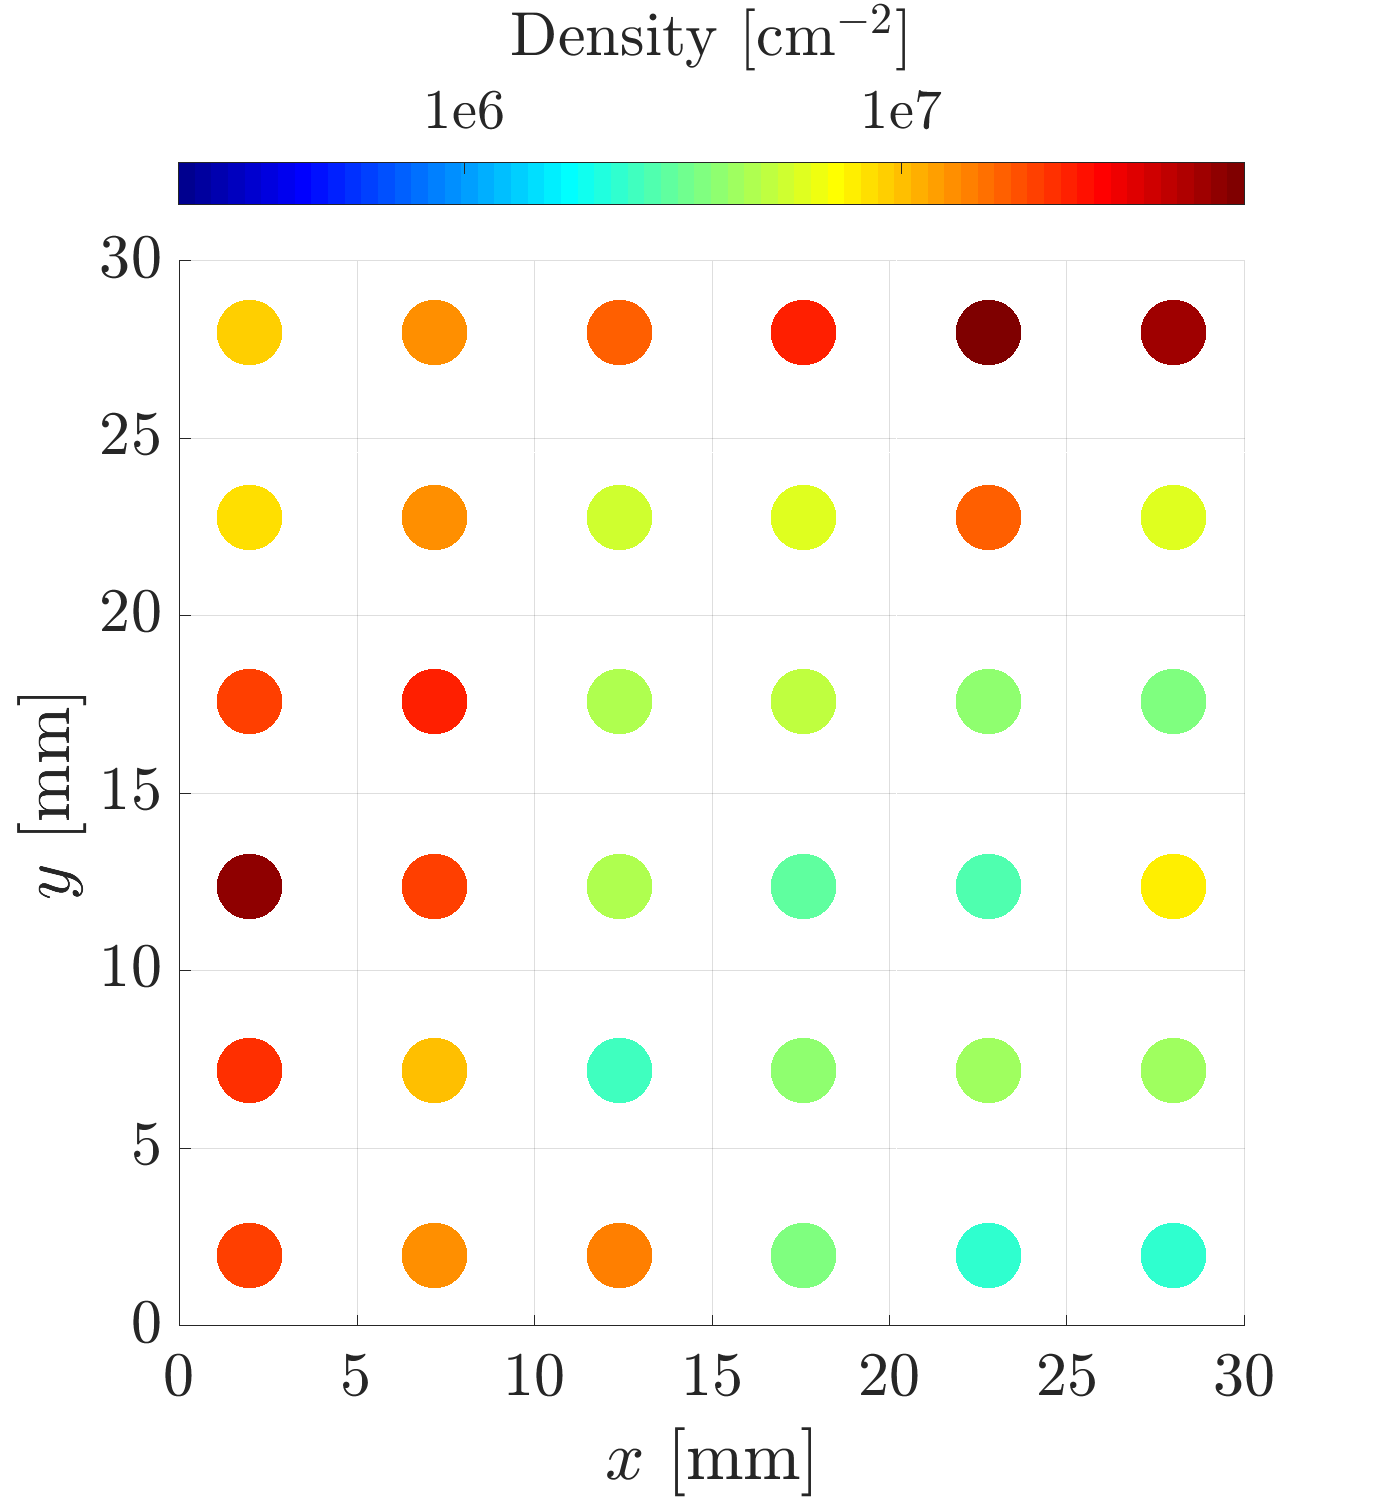
\includegraphics[width=\linewidth]{subB2b_densityData.png}
        \caption{Substrate B2 with surface pre-growth preparation.}\label{fig:subB2b_densityData}
    \end{subfigure}
    \caption[Map of the polishing grit density on substrate B and B2 after surface pre-growth preparation.]{A map of the polishing grit density on the $\SI{30}{\milli\metre}\times\SI{30}{\milli\metre}$ substrates B and B2 after surface pre-growth preparation. Counts are taken from 121 different locations on B and 36 different locations on B2. The polishing grit density was observed to vary between \SI{5e+06}{\particle\centi\metre^{-2}} and \SI{5e+07}{\particle\centi\metre^{-2}}.}
    \label{fig:subBb_and_subB2b_densityData}
\end{figure}

In order to observe correlations between the occurrence of voids and microvoids on the as-received substrate B to the occurrence of polishing grit after polish and etch, the sample Pearson correlation coefficient was determined. \todo{Skriv inn formel. Og regn ut correlation.} If there are one dataset $x_i \in \{x_1, ..., x_n\}$ containing $n$ values and another dataset $y_i \in \{y_1, ..., y_n\}$ containg $n$ values, then the sample Pearson correlation coefficient is defined as

\begin{equation}\label{eq:pearson_correlation_coefficient}
    r = \frac{
        n\sum_{i=1}^nx_iy_i - \sum_{i=1}^n x_i \sum_{i=1}^n y_i
        }{
        \sqrt{n\sum_{i=1}^n x_i^2 - \parentheses{\sum_{i=1}^n x_i}^2}\sqrt{n\sum_{i=1}^n y_i^2 - \parentheses{\sum_{i=1}^n y_i}^2} },
\end{equation}
where $\avg{x}=\frac{1}{n}\sum_{i=1}^n x_i$ is the sample mean; and analogously for $\avg{y}$.
%
%\begin{equation}
%    r = \frac{\sum_{i=1}^n x_i y_i - n\avg{x}\avg{y}}{\parentheses{n-1}s_xs_y},
%\end{equation}
%where $s_x = \sqrt{\frac{1}{n-1}\sum_{i=1}^n \parentheses{x_i - \avg{x}}^2}$ is the sample standard deviation; and analogously for $s_y$.


%%=========================================
%\section{AFM Study of Polished and Etched Substrate B}
\subsection{Surface Roughness}
Fig.~\ref{fig:subBb_and_subB2_afm} or Fig~\ref{fig:subBb_afm_centre}--\subref{fig:subBb_afm_corner} substrate B; and Fig.~\ref{fig:subB2b_afm_centre}--\subref{fig:subB2b_afm_corner} substrate B2.

\begin{figure}[htbp]
    \centering
    \begin{subfigure}[t]{0.3\linewidth}
    \centering
        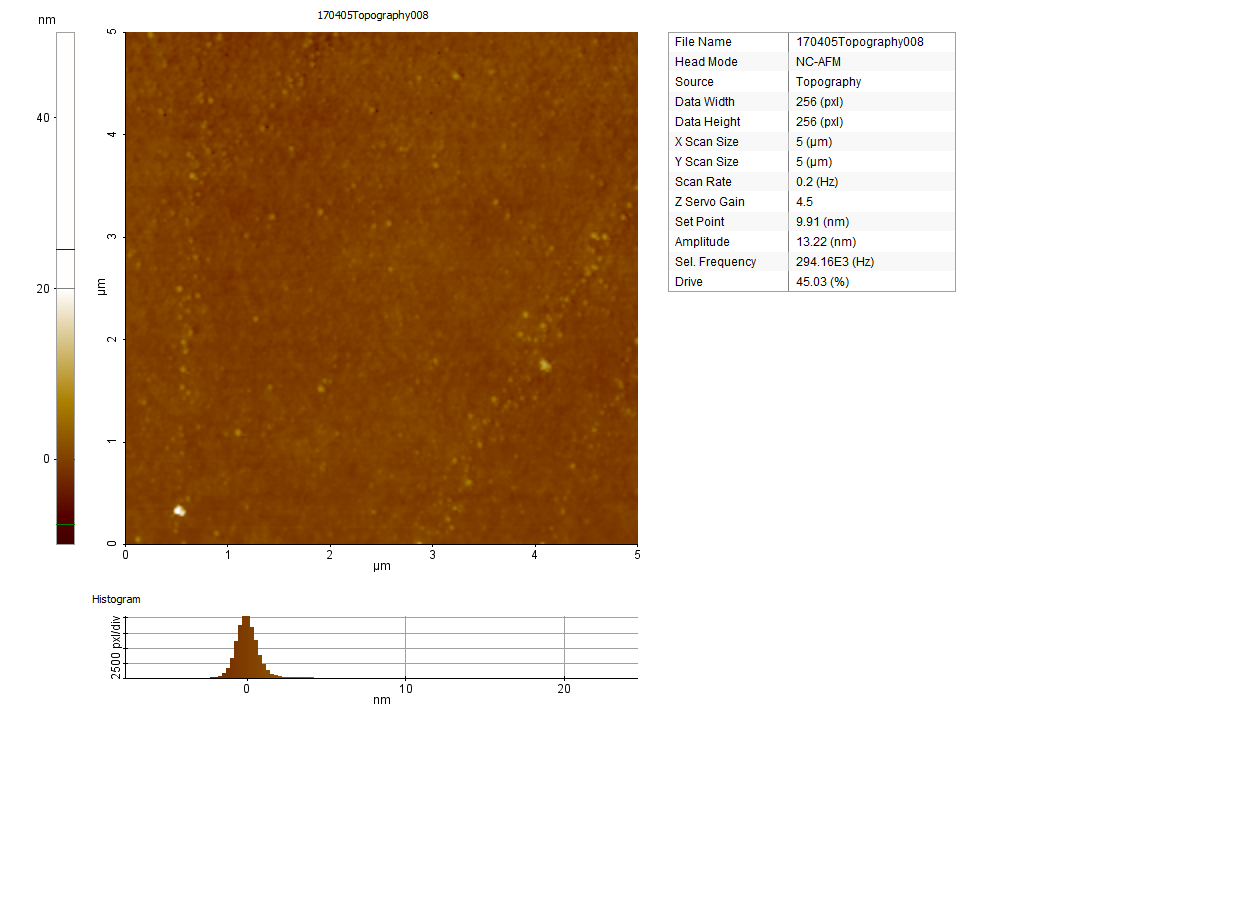
\includegraphics[width=\linewidth,trim={0cm 12cm 21cm 0cm},clip]{170405Topography008_centre.png}
        \caption{}\label{fig:subBb_afm_centre}%\SI{0.85}{\nano\metre}
    \end{subfigure}%
    \hfill
    \begin{subfigure}[t]{0.3\linewidth}
    \centering
        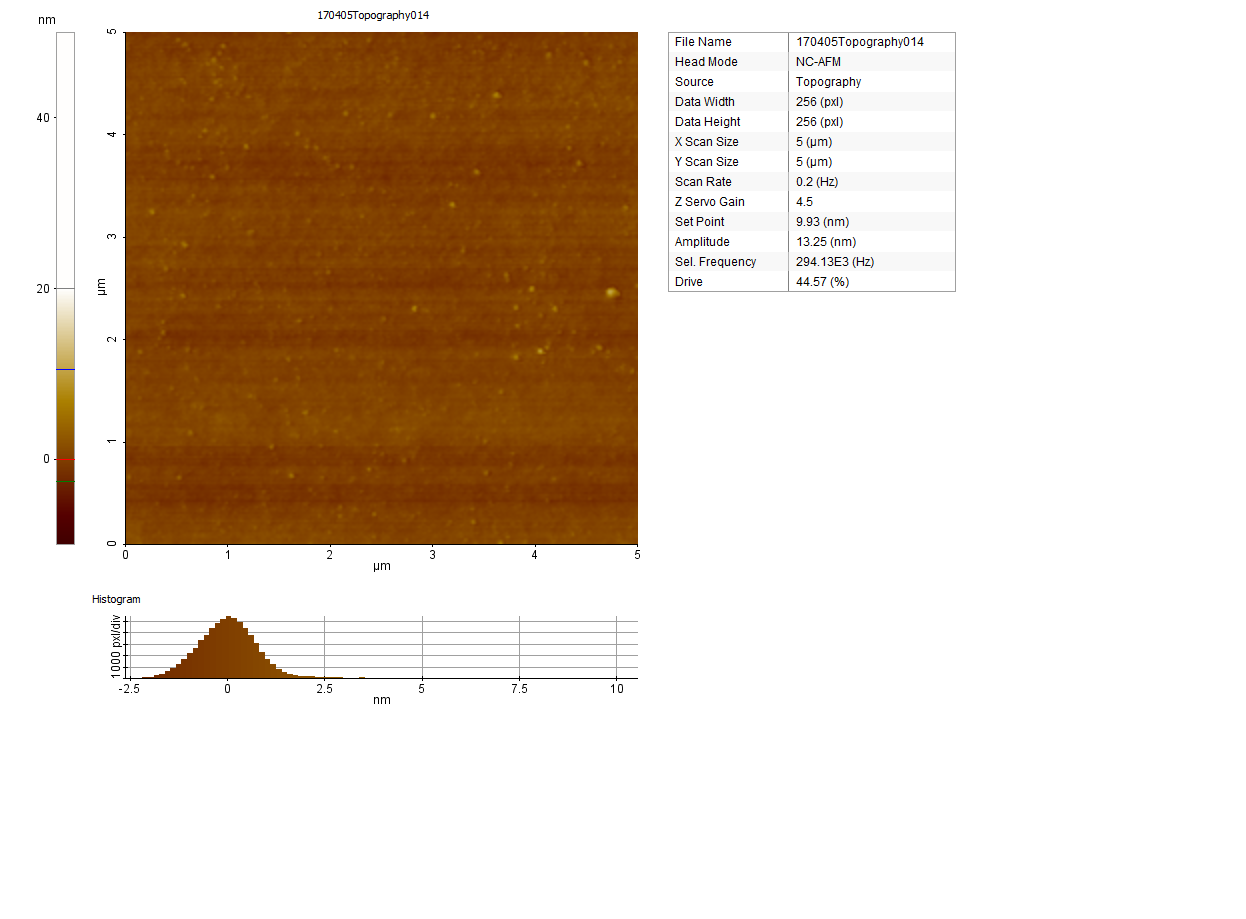
\includegraphics[width=\linewidth,trim={0cm 12cm 21cm 0cm},clip]{170405Topography014_leftedge.png}
        \caption{}\label{fig:subBb_afm_edge}%\SI{0.77}{\nano\metre}
    \end{subfigure}%
    \hfill
    \begin{subfigure}[t]{0.3\linewidth}
    \centering
        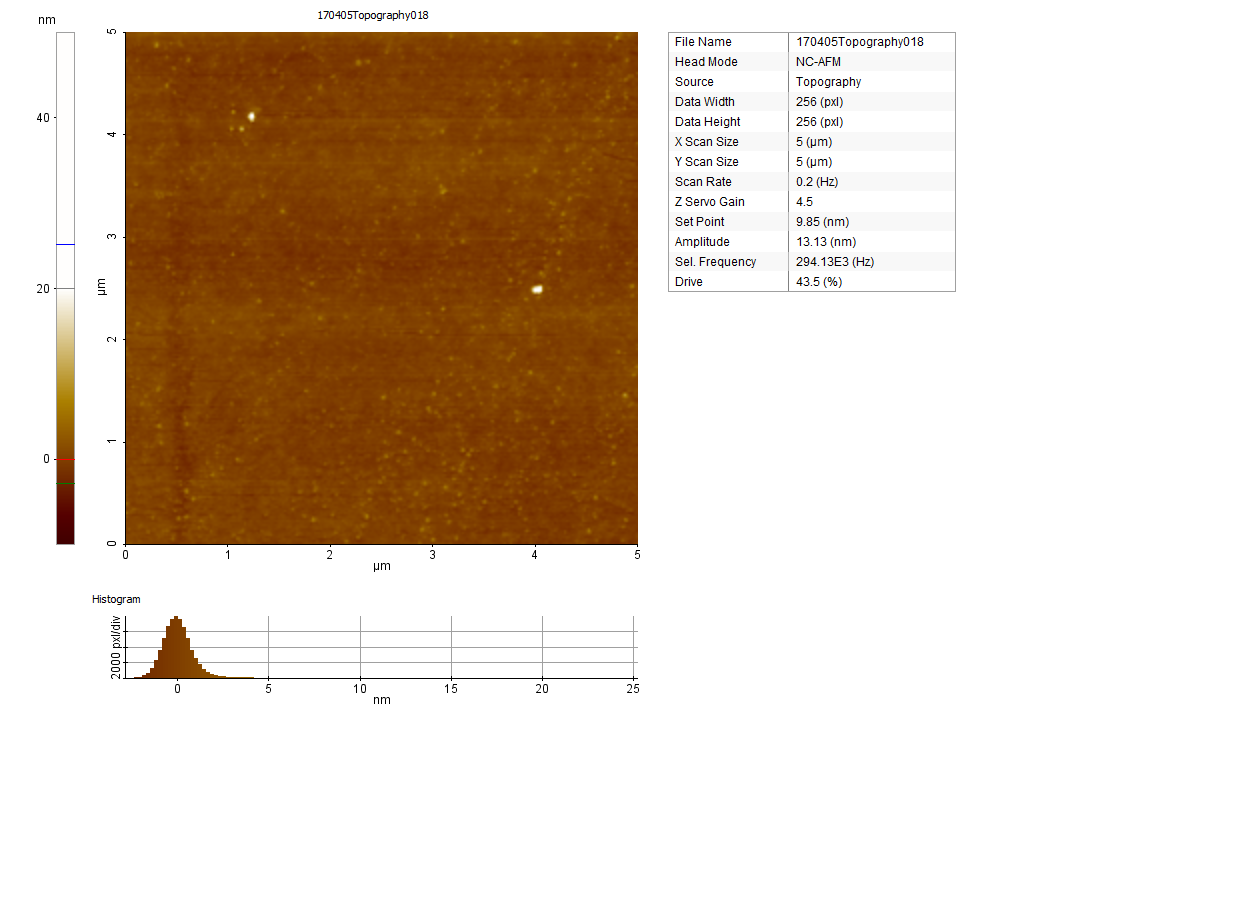
\includegraphics[width=\linewidth,trim={0cm 12cm 21cm 0cm},clip]{170405Topography018_upperleftcorner.png}
        \caption{}\label{fig:subBb_afm_corner} %\SI{1,04}{\nano\metre}}
    \end{subfigure}%
    \par\bigskip
    \begin{subfigure}[t]{0.3\linewidth}
    \centering
        
\includegraphics[width=\linewidth,trim={0cm 12cm 21cm 0cm},clip]{unknown.png}
        \caption{}\label{fig:subB2b_afm_centre}
    \end{subfigure}%
    \hfill
    \begin{subfigure}[t]{0.3\linewidth}
    \centering
        
\includegraphics[width=\linewidth,trim={0cm 12cm 21cm 0cm},clip]{unknown.png}
        \caption{}\label{fig:subB2b_afm_edge}
    \end{subfigure}%
    \hfill
    \begin{subfigure}[t]{0.3\linewidth}
    \centering
        
\includegraphics[width=\linewidth,trim={0cm 12cm 21cm 0cm},clip]{unknown.png}
        \caption{}\label{fig:subB2b_afm_corner} 
    \end{subfigure}%
    \caption[\Ac{afm} of substrate B and substrate B2 with surface pre-growth preparation.]{\Acf{afm} measurements of substrate B and substrate B2 with surface pre-growth preparation. Images of $\SI{5}{\micro\metre}\times\SI{5}{\micro\metre}$ areas are taken at three different locations on the substrate surfaces. For substrate B: \subref{fig:subBb_afm_centre} near the centre, \ac{rms} roughness \SI{0.85}{\nano\metre}; \subref{fig:subBb_afm_edge} near the left edge, \ac{rms} roughness \SI{0.76}{\nano\metre}; and \subref{fig:subBb_afm_corner} near the upper left corner, \ac{rms} roughness \SI{0.92}{\nano\metre}. For substrate B2: \subref{fig:subB2b_afm_centre} near the centre, \ac{rms} roughness \SI{0.91}{\nano\metre}; \subref{fig:subB2b_afm_edge} near the upper edge, \ac{rms} roughness \SI{0.96}{\nano\metre}; and \subref{fig:subB2b_afm_corner} near the upper left corner, \ac{rms} roughness \SI{1.3}{\nano\metre}.}\label{fig:subBb_and_subB2_afm}
\end{figure} % AFM, substrate B, with surface pre-growth preparation.

% B2: AFM: UL - 1.310 nm, U-edge - 0.956, Centre- 0.912 nm

%%=========================================
\subsection{Impurity Analysis}
\begin{table}[htbp]
    \centering
    \caption[\Ac{eds} impurity analysis of substrate B with surface pre-growth preparation.]{Results of the \acf{eds} impurity analysis at three different locations on the $30\times30$ \SI{}{\milli\metre^2} (111)B \ac{czt} substrate B with surface pre-growth preparation (atomic concentration \%). The X-ray signal is acquired from $\SI{1270}{\micro\metre}\times\SI{890}{\micro\metre}$ areas near the centre, upper edge, and upper left corner.}\label{tab:subBb_eds_analysis}
    \begin{tabu} to 1.0\textwidth { X[1.85,r] X[1.125,c] X[1.125,c] X[1.125,c] X[1.125,c] X[1.125,c] X[1.125,c] X[1.125,c] }
    \hline
         & \textbf{\ce{Te}} (at.\%) & \textbf{\ce{Cd}} (at.\%) & \textbf{\ce{Zn}} (at.\%) & \textbf{\ce{Al} } (at.\%) & \textbf{\ce{Si}} (at.\%) & \textbf{\ce{C}} (at.\%) & \textbf{\ce{O}} (at.\%) \\
        \hline
        Near centre  & \SI{46.10}{} & \SI{45.35}{} & \SI{1.92}{} & \SI{0.23}{} & \SI{0.52}{} & \SI{5.49}{} & \SI{0.40}{} \\ % \SI{15.0}{} & \SI{15.0}{}
        Near edge & \SI{45.49}{} & \SI{45.12}{} & \SI{2.02}{} & \SI{0.26}{} & \SI{0.49}{} & \SI{5.99}{} & \SI{0.64}{} \\ % \SI{15.0}{} & \SI{29.0}{}
        Near corner & \SI{45.83}{} & \SI{45.34}{} & \SI{1.92}{} & \SI{0.60}{} & \SI{0.50}{} & \SI{5.34}{} & \SI{0.47}{} \\ % \SI{1.0}{}  & \SI{29.0}{}
         \hline
    \end{tabu}
\end{table}
%%=========================================
% FTIR transmission spectra.
\subsection{IR Characterisation}



%%=========================================
